\chapter{DNA 复制}\label{ch:g11:dna-replication}

你的骨髓每天生成两千亿个新的红\omterm{def:g10:cells-common-unit:cell}{细胞}，你的肠道内壁每隔几天便更新一次，
而每一个新\omterm{def:g10:cells-common-unit:cell}{细胞}都会获得一份完整的
两米长的 \omterm{def:g10:universal-dna:information}{DNA} 拷贝，前几章把它描述为\omterm{def:g10:cells-common-unit:cell}{细胞}的“文本”。
在没有可供查对的模板的情况下，
要在几小时内复制三十亿个碱基，
错误率却低于专业打字员每页的错误数：这是怎样做到的？
答案早在 1953 年便由分子本身的结构推测得出，
并于五年后
被生物学中最精妙的实验之一所证实。

\section{复制的问题}

\begin{definition}[复制]\label{def:g11:dna-replication:replication}
\emph{DNA 复制}\index{DNA 复制}是指\omterm{def:g10:cells-common-unit:cell}{细胞}在分裂前，
由一个双链 \omterm{def:g10:universal-dna:information}{DNA} 分子产生两个相同分子的过程，
这两个分子与原分子及彼此完全相同。它发生在\omterm{def:g10:cells-common-unit:cell}{细胞}周期的一个特定时期，
即 \emph{S 期}
（\cref{ch:g11:cell-cycle-mitosis}），在此期间\omterm{def:g10:cells-common-unit:organelle}{细胞核}中的 \omterm{def:g10:universal-dna:information}{DNA} 含量
加倍。
\end{definition}

\begin{proposition}[模板原理]\label{prop:g11:dna-replication:template}
由于 \omterm{def:g10:universal-dna:information}{DNA} 分子的两条链互补——A 与 T 相对，
G 与 C 相对——每条链都携带重建另一条链所需的全部信息，
因此，复制时先将两条链分开，
以每条链为\emph{模板}，
逐个\omterm{def:g10:universal-dna:nucleotide}{核苷酸}组装出一条新的互补链。
\end{proposition}
\admitted

\begin{example}[三种可能的结果]\label{ex:g11:dna-replication:models}
根据模板原理，人们在 1950 年代提出了三种
新旧链的分布方式：
\begin{itemize}
  \item \emph{半保留复制}：每个子代分子保留
        一条旧链，并获得一条新链；
  \item \emph{全保留复制}：原分子整体保留，
        并在其旁边合成一条全新的双链；
  \item \emph{分散复制}：新旧片段沿
        两个子代分子的每条链交替排列。
\end{itemize}
仅靠观察无法区分三者，称量却可以。
\end{example}

\section{梅塞尔森–斯塔尔实验}

\begin{proposition}[复制是半保留的]\label{prop:g11:dna-replication:semiconservative}
每个子代 \omterm{def:g10:universal-dna:information}{DNA} 分子含有一条亲代链，
和一条新合成的链。
\end{proposition}
\begin{proof}[证据]
梅塞尔森与斯塔尔（1958 年）将细菌培养多代，所用培养基
中唯一的氮源是重同位素 $^{15}$N，以致细菌的全部 \omterm{def:g10:universal-dna:information}{DNA} 均为重型。
随后他们将细菌转入普通的
$^{14}$N 培养基中培养，并在每代之后取样
（每代二十分钟）。将每份样品提取的 \omterm{def:g10:universal-dna:information}{DNA} 在浓盐溶液中离心
数小时，分子会漂浮在与自身密度相当的液面位置，
然后在紫外线下拍照：
重 \omterm{def:g10:universal-dna:information}{DNA} 与轻 \omterm{def:g10:universal-dna:information}{DNA} 形成条带，两条带之间的距离可以测量。
结果：转移前，只有一条重带；一代之后，
仅有一条恰好位于重带与轻带之间的条带——每个分子都是杂合的；
两代之后，出现两条量相等的条带，
一条为杂合，一条为轻；三代之后，轻带的量
为杂合带的三倍。全保留模型预测第一代即出现一条重带和一条轻带，
而不会出现杂合带；分散模型预测只有一条条带，
每代都向轻的方向漂移，永不分裂为两条；
只有半保留模型给出第一代一条杂合带，
随后出现杂合带与轻带，比例与观测结果相符。
\end{proof}

\begin{omfigure}
\begin{tikzpicture}[font=\small]
  \tikzset{tube/.style={draw, thick, rounded corners=6pt, minimum width=1.3cm, minimum height=3.6cm}}
  \foreach \x/\g in {0/{第 0 代}, 3/{第 1 代}, 6/{第 2 代}, 9/{第 3 代}} {
    \node[tube] (t\x) at (\x,0) {};
    \node[anchor=north, align=center] at (\x,-1.95) {\g};
  }
  \draw[dashed, gray] (-1.0,1.2) -- (10.6,1.2) node[right, gray] {轻};
  \draw[dashed, gray] (-1.0,0.0) -- (10.6,0.0) node[right, gray] {杂合};
  \draw[dashed, gray] (-1.0,-1.2) -- (10.6,-1.2) node[right, gray] {重};
  % bands: width encodes intensity
  \fill[omDef] (-0.55,-1.28) rectangle (0.55,-1.12);
  \fill[omDef] (2.45,-0.08) rectangle (3.55,0.08);
  \fill[omDef] (5.45,-0.06) rectangle (6.55,0.06);
  \fill[omDef] (5.45,1.14) rectangle (6.55,1.26);
  \fill[omDef] (8.45,-0.03) rectangle (9.55,0.03);
  \fill[omDef] (8.45,1.11) rectangle (9.55,1.29);
  \node[anchor=south, align=center] at (4.5,2.0) {离心后密度梯度中的 DNA 条带};
\end{tikzpicture}

{\small 梅塞尔森–斯塔尔实验结果。转移前为重 \omterm{def:g10:universal-dna:information}{DNA}；
在轻培养基中培养一代后，只有一条杂合带；
两代后，杂合与轻 \omterm{def:g10:universal-dna:information}{DNA} 的量相等；三代后，轻 \omterm{def:g10:universal-dna:information}{DNA} 为杂合的三倍。
条带粗细表示 \omterm{def:g10:universal-dna:information}{DNA} 的量。}
\end{omfigure}

\begin{omfigure}
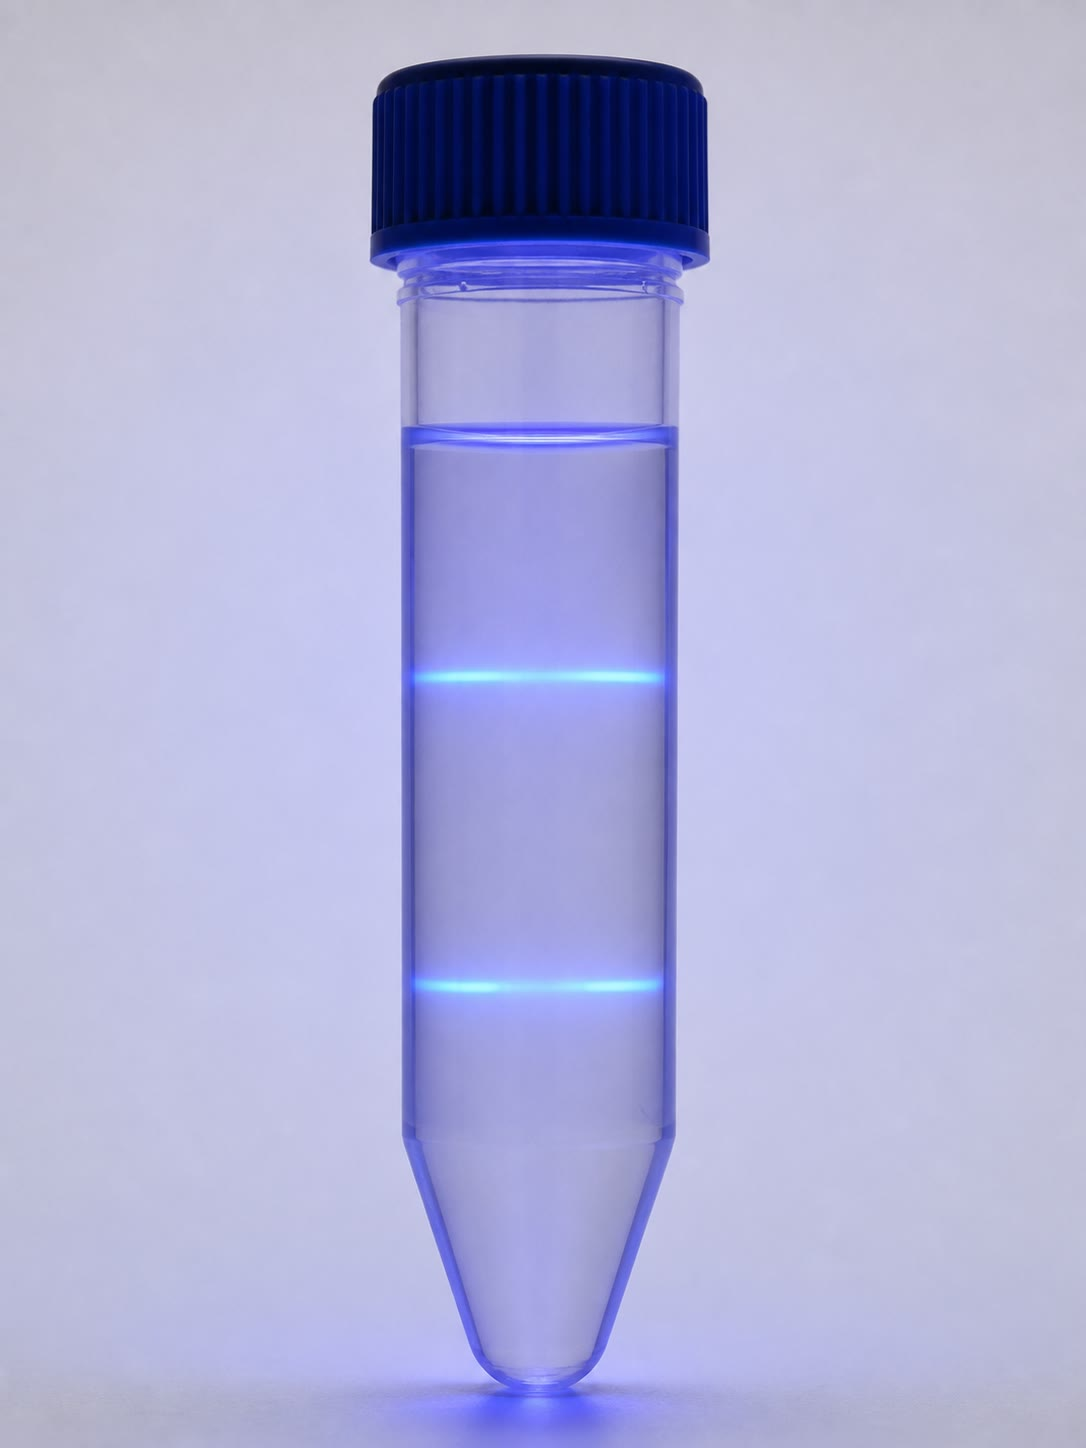
\includegraphics[width=0.3\linewidth]{images/book2/ai/g11-replication-centrifuge-tube.jpg}

{\small 紫外线下的离心管：两种密度的 \omterm{def:g10:universal-dna:information}{DNA} 分子
已漂浮至盐梯度中的两个高度，并呈现为
两条条带。条带的位置可测量其密度，亮度
则反映其含量。}
\end{omfigure}

\begin{example}[预测第四代]\label{ex:g11:dna-replication:fourth}
在轻培养基中培养 $n$ 代后，原有的两条重链
仍然存在，各位于两个杂合分子中；其余分子
全部为轻分子。在 $2^n$ 个分子中，2 个为杂合，
$2^n - 2$ 个为轻；第 4 代时，2 个杂合对 14 个轻——轻带的量
为杂合带的七倍，而杂合带永远不会消失，
只会变淡。两条原始链实际上可以说是“永生”的。
\end{example}

\section{复制机制}

\begin{proposition}[复制叉]\label{prop:g11:dna-replication:forks}
复制始于确定的位点，即\emph{复制起点}，两条链在该处
被拆开形成一个泡。在泡的每一端，一个
\emph{复制叉}\index{复制叉}推进：一种酶，
\emph{DNA 聚合酶}\index{DNA 聚合酶}，沿每条被打开的
单链逐个加入与之互补的\omterm{def:g10:universal-dna:nucleotide}{核苷酸}，
并将其连接到新链上。泡的两个\omterm{prop:g11:dna-replication:forks}{复制叉}朝相反
方向移动，直至与相邻泡的\omterm{prop:g11:dna-replication:forks}{复制叉}相遇；
细菌\omterm{def:g10:universal-dna:information}{染色体}是单个环状分子，只有一个复制起点和两个
\omterm{prop:g11:dna-replication:forks}{复制叉}；人类\omterm{def:g10:universal-dna:information}{染色体}则同时有数千个复制起点在工作。
\end{proposition}
\admitted

\begin{omfigure}
\begin{tikzpicture}[font=\small, >=Stealth, line cap=round]
  % parent strands
  \draw[very thick, omDef] (0,0.5) -- (4,0.5);
  \draw[very thick, omDef] (0,-0.5) -- (4,-0.5);
  \draw[very thick, omDef] (4,0.5) .. controls (5.5,0.5) and (6,1.4) .. (8.5,1.6);
  \draw[very thick, omDef] (4,-0.5) .. controls (5.5,-0.5) and (6,-1.4) .. (8.5,-1.6);
  % new strands
  \draw[very thick, omThm] (4.4,0.35) .. controls (5.6,0.4) and (6,1.0) .. (8.5,1.2);
  \draw[very thick, omThm] (4.4,-0.35) .. controls (5.6,-0.4) and (6,-1.0) .. (8.5,-1.2);
  % base pair rungs (parent)
  \foreach \x in {0.3,0.7,...,3.9} \draw[gray] (\x,0.5) -- (\x,-0.5);
  % rungs in daughter helices
  \foreach \t in {0.15,0.3,...,0.95} {
    \draw[gray] ({4+4.5*\t},{0.5+1.1*\t*\t+0.0}) -- ({4+4.5*\t},{0.35+0.85*\t*\t});
    \draw[gray] ({4+4.5*\t},{-0.5-1.1*\t*\t}) -- ({4+4.5*\t},{-0.35-0.85*\t*\t});
  }
  % polymerases
  \node[draw, fill=omProp!35, circle, minimum size=0.55cm, inner sep=0] (p1) at (6.6,0.95) {};
  \node[draw, fill=omProp!35, circle, minimum size=0.55cm, inner sep=0] (p2) at (6.6,-0.95) {};
  \node[anchor=south, align=center] at (6.6,2.0) {DNA 聚合酶};
  \draw[->] (6.6,1.95) -- (p1.north);
  \draw[->] (6.6,-1.95) -- (p2.south);
  \node[anchor=north, align=center] at (6.6,-2.05) {DNA 聚合酶};
  % labels
  \node[anchor=east, omDef, align=right] at (-0.15,0) {亲代 \\双链};
  \node[anchor=west, align=left] at (8.7,1.4) {子代 1};
  \node[anchor=west, align=left] at (8.7,-1.4) {子代 2};
  \draw[->, thick] (2.0,-1.5) -- (3.9,-1.5) node[midway, below] {复制叉移动};
  \node[omDef, anchor=south west] at (0.1,0.6) {旧链};
  \node[omThm, anchor=north west] at (5.6,-0.05) {新链};
\end{tikzpicture}

{\small \omterm{prop:g11:dna-replication:forks}{复制叉}示意图。亲代链（蓝色）分开；在每条链上，
一个 \omterm{def:g10:universal-dna:information}{DNA} 聚合酶合成一条新的互补链（红色）。\omterm{prop:g11:dna-replication:forks}{复制叉}之后
为两段双链，每段各含一条旧链和一条新链。}
\end{omfigure}

\begin{example}[速度与规模]\label{ex:g11:dna-replication:speed}
细菌\omterm{prop:g11:dna-replication:forks}{复制叉}每秒约添加 1000 个\omterm{def:g10:universal-dna:nucleotide}{核苷酸}；人类\omterm{prop:g11:dna-replication:forks}{复制叉}约
为 50 个。\emph{E.~coli} \omterm{def:g10:universal-dna:information}{染色体}含 $\num{4.6e6}$ 个碱基对，
由一个复制起点出发的两个\omterm{prop:g11:dna-replication:forks}{复制叉}复制，需要 $\num{4.6e6}/(2 \times
1000) \approx \qty{2300}{s}$，约 40 分钟——这正是
该细菌在富营养培养基中的\omterm{def:g10:cells-common-unit:cell}{细胞}周期长度。人类\omterm{def:g10:cells-common-unit:cell}{细胞}含 $\num{6.4e9}$
碱基对需要复制，S 期约 8 小时，需要数千个
复制起点；单个\omterm{prop:g11:dna-replication:forks}{复制叉}则需两年多。
\end{example}

\begin{omfigure}
\begin{tikzpicture}[font=\small, >=Stealth]
  \foreach \y/\lab in {0/{S 期开始}, -1.4/{稍后}, -2.8/{S 期结束}} {
    \node[anchor=east] at (-0.3,\y) {\lab};
  }
  % row 1: single line with origins marked
  \draw[very thick, omDef] (0,0) -- (10,0);
  \foreach \x in {1.5,4,6.5,9} \fill[omThm] (\x,0) circle (2pt);
  \node[anchor=west, font=\scriptsize] at (10.1,0) {复制起点};
  % row 2: bubbles
  \draw[very thick, omDef] (0,-1.4) -- (10,-1.4);
  \foreach \x/\w in {1.5/0.7, 4/0.9, 6.5/0.6, 9/0.5} {
    \draw[very thick, omDef, fill=white] (\x-\w,-1.4) .. controls (\x-\w/2,-1.05) and (\x+\w/2,-1.05) .. (\x+\w,-1.4)
      .. controls (\x+\w/2,-1.75) and (\x-\w/2,-1.75) .. (\x-\w,-1.4);
    \draw[very thick, omThm] (\x-\w+0.05,-1.4) .. controls (\x-\w/2,-1.15) and (\x+\w/2,-1.15) .. (\x+\w-0.05,-1.4);
    \draw[very thick, omThm] (\x-\w+0.05,-1.4) .. controls (\x-\w/2,-1.65) and (\x+\w/2,-1.65) .. (\x+\w-0.05,-1.4);
    \draw[->, thick] (\x-\w-0.05,-1.4) -- (\x-\w-0.45,-1.4);
    \draw[->, thick] (\x+\w+0.05,-1.4) -- (\x+\w+0.45,-1.4);
  }
  % row 3: two full molecules
  \draw[very thick, omDef] (0,-2.65) -- (10,-2.65);
  \draw[very thick, omThm] (0,-2.8) -- (10,-2.8);
  \draw[very thick, omThm] (0,-3.0) -- (10,-3.0);
  \draw[very thick, omDef] (0,-3.15) -- (10,-3.15);
  \node[anchor=west, font=\scriptsize, align=left] at (10.1,-2.9) {两个拷贝};
\end{tikzpicture}

{\small 长\omterm{def:g10:universal-dna:information}{染色体}由多个复制起点同时复制。泡
在复制起点处打开，每个泡有两个相背移动的\omterm{prop:g11:dna-replication:forks}{复制叉}；泡不断扩大、相遇，
最终合并，形成两条完整的双链，每条一半为旧链（蓝色），
一半为新链（红色）。}
\end{omfigure}

\begin{proposition}[复制保真性]\label{prop:g11:dna-replication:fidelity}
\omterm{def:g10:universal-dna:information}{DNA} 聚合酶配错\omterm{def:g10:universal-dna:nucleotide}{核苷酸}的概率约为 $10^5$ 分之一；它在
每加入一个\omterm{def:g10:universal-dna:nucleotide}{核苷酸}时即进行校对，并一次性清除大部分错配，
其余大部分错配则由其他酶在\omterm{prop:g11:dna-replication:forks}{复制叉}后方纠正，
最终错误率约为每 $10^9$ 个\omterm{def:g10:universal-dna:nucleotide}{核苷酸}一次；
人类\omterm{def:g10:cells-common-unit:cell}{细胞}复制 $\num{6.4e9}$ 个\omterm{def:g10:universal-dna:nucleotide}{核苷酸}，平均每次分裂
约出现六个错误。未被纠正的错误即为
\emph{突变}，在\cref{ch:g11:mutations}中讨论。
\end{proposition}
\admitted

\begin{method}[复制计算]\label{met:g11:dna-replication:calc}
\begin{enumerate}
  \item \emph{时间}：复制长度（碱基对数）除以所有
        正在工作的所有\omterm{prop:g11:dna-replication:forks}{复制叉}的总速度（\omterm{prop:g11:dna-replication:forks}{复制叉}数 $\times$ 每叉每秒
        添加的\omterm{def:g10:universal-dna:nucleotide}{核苷酸}数）。
  \item \emph{所需复制起点数}：总长度除以一个复制起点
        （两个\omterm{prop:g11:dna-replication:forks}{复制叉}）在可用时间内所能复制的长度。
  \item \emph{错误数}：复制的\omterm{def:g10:universal-dna:nucleotide}{核苷酸}数 $\times$ 错误率；
        注意\omterm{def:g10:cells-common-unit:cell}{细胞}复制两条链，即碱基对数的
        两倍。
  \item \emph{同位素实验}：追踪两条原始链；
        经过 $n$ 代后，它们位于 $2^n$ 个分子中的
        2 个杂合分子中。
\end{enumerate}
\end{method}

\begin{remark}[结构与机制为何吻合]\label{rem:g11:dna-replication:fit}
沃森和克里克在 1953 年的论文末尾指出，这种配对
“立即提示了一种可能的复制机制”。梅塞尔森和斯塔尔
证明这确实是真实的机制；随后的酶学研究
阐明了具体过程。这是生物学中少有的例子之一，即一种分子的
结构一经看清，便决定了使用它的过程。
\end{remark}

\section{练习}

\begin{exercise}[$\star$]\label{exo:g11:dna-replication:1}
说明模板原理，并解释它为何依赖于
\omterm{prop:g10:universal-dna:helix}{互补性}。
\end{exercise}

\begin{exercise}[$\star$]\label{exo:g11:dna-replication:2}
给出半保留复制的定义，并将其与
保守模型进行比较。
\end{exercise}

\begin{exercise}[$\star$]\label{exo:g11:dna-replication:3}
复制发生在\omterm{def:g10:cells-common-unit:cell}{细胞}周期的哪一时期？其间
每个\omterm{def:g10:cells-common-unit:organelle}{细胞核}中的 \omterm{def:g10:universal-dna:information}{DNA} 量发生了怎样的变化？
\end{exercise}

\begin{exercise}[$\star$]\label{exo:g11:dna-replication:4}
\omterm{def:g10:universal-dna:information}{DNA} 聚合酶的作用是什么？\omterm{prop:g11:dna-replication:forks}{复制叉}是什么？
\end{exercise}

\begin{exercise}[$\star$]\label{exo:g11:dna-replication:5}
一条链的序列为 \texttt{GATTACAGGC}，写出聚合酶
以它为模板合成的新链。
\end{exercise}

\begin{exercise}[$\star\star$]\label{exo:g11:dna-replication:6}
在梅塞尔森–斯塔尔实验中，
保守模型在第 1 代会预测什么，分散模型在第 2 代又会预测什么？
二者各自为何不能成立？
\end{exercise}

\begin{exercise}[$\star\star$]\label{exo:g11:dna-replication:7}
预测第 5 代时的条带及其相对强度。
\end{exercise}

\begin{exercise}[$\star\star$]\label{exo:g11:dna-replication:8}
将在轻培养基中培养的细菌转移到重培养基中。
描述第 0、1 和 2 代时的条带。
\end{exercise}

\begin{exercise}[$\star\star$]\label{exo:g11:dna-replication:9}
计算单个人类\omterm{prop:g11:dna-replication:forks}{复制叉}以每秒 50 个\omterm{def:g10:universal-dna:nucleotide}{核苷酸}的速度
复制一条含 $\num{2.5e8}$ 个碱基对的\omterm{def:g10:universal-dna:information}{染色体}所需的时间，并与
持续 8 小时的 S 期进行比较，并作出结论。
\end{exercise}

\begin{exercise}[$\star\star$]\label{exo:g11:dna-replication:10}
一个人类\omterm{def:g10:cells-common-unit:cell}{细胞}在一个 S 期内共连接了多少
个\omterm{def:g10:universal-dna:nucleotide}{核苷酸}？若每 $10^9$ 个\omterm{def:g10:universal-dna:nucleotide}{核苷酸}出现 1 个错误，则它会出现多少个错误？
\end{exercise}

\begin{exercise}[$\star\star$]\label{exo:g11:dna-replication:11}
为什么一个复制泡的两个\omterm{prop:g11:dna-replication:forks}{复制叉}必须沿相反方向移动？
相邻两个复制泡相遇时又会发生什么？
\end{exercise}

\begin{exercise}[$\star\star\star$]\label{exo:g11:dna-replication:12}
某种化学物质会阻断 \omterm{def:g10:universal-dna:information}{DNA} 聚合酶。预测它对细菌
培养物、正在愈合的伤口以及不再
分裂的神经\omterm{def:g10:cells-common-unit:cell}{细胞}的影响。哪一种影响提示了它在医学上的用途？
\end{exercise}

\begin{exercise}[$\star\star\star$]\label{exo:g11:dna-replication:13}
在梅塞尔森–斯塔尔实验中，杂合条带从未消失。
请解释原因，并计算经过
10 代后杂合分子所占的比例。
\end{exercise}

\begin{exercise}[$\star\star\star$]\label{exo:g11:dna-replication:14}
一种不具备校对活性的聚合酶，每 $10^5$ 个\omterm{def:g10:universal-dna:nucleotide}{核苷酸}出现 1 个错误。
计算在无校对的情况下，每次人类\omterm{def:g10:cells-common-unit:cell}{细胞}分裂产生的错误数，并
解释为何这样的\omterm{def:g10:cells-common-unit:cell}{细胞}系无法经过多次分裂后仍能存活。
\end{exercise}

\begin{exercise}[$\star\star\star$]\label{exo:g11:dna-replication:15}
解释为何富营养培养基中的细菌能每 20 分钟分裂一次，
尽管复制其\omterm{def:g10:universal-dna:information}{染色体}需要 40 分钟。（提示：想一想
下一轮复制何时可以开始。）
\end{exercise}

\section{问题：称量分子以观察其复制}

\begin{problem}[{周末问题——重建梅塞尔森–斯塔尔实验：同位素、
三种模型及其预测、起决定作用的条带，以及
能在 40 分钟内复制一条染色体的复制叉
}]
\label{pb:g11:dna-replication:1}
普通氮为 $^{14}$N；重同位素 $^{15}$N 每个原子
重 7\%。氮约占 \omterm{def:g10:universal-dna:information}{DNA} 质量的 16\%。
将在 $^{15}$N 培养基中培养 14 代的细菌，于零时刻
转移到 $^{14}$N 培养基中，并每 20 分钟分裂一次。

\medskip
\noindent\textbf{第一部分——重与轻。}
\begin{enumerate}
  \item 完全重型 \omterm{def:g10:universal-dna:information}{DNA} 的密度比轻型 \omterm{def:g10:universal-dna:information}{DNA} 高出多少比例？
        （假设密度与质量成正比。）为何这样微小的差异
        就足以将条带分离开？
  \item 为何要让细菌先在重培养基中培养 14 代
        之后才转移，而不是培养一代或两代？
  \item 一个杂合分子含有一条重链和一条轻链。
        它会漂浮在重条带与轻条带的什么位置？
  \item 解释为何必须从大量细菌中提取 \omterm{def:g10:universal-dna:information}{DNA}，才能
        使条带可以被看到。
  \item 实验者如何能确定，转移至轻培养基的操作
        本身并未改变细菌的 \omterm{def:g10:universal-dna:information}{DNA}？
\end{enumerate}

\medskip
\noindent\textbf{第二部分——三种预测。}
  对每种模型，给出经过一代和两代后预期的条带
        （位置与相对量）。
\begin{enumerate}[resume]
  \item 半保留复制模型。
  \item 全保留复制模型。
  \item 弥散复制模型。
  \item 一代后只出现一条位于重带与轻带
        正中间的条带。哪一种模型被立即排除，
        余下哪两种？
  \item 两代后出现两条条带，即杂合带与轻带，
        强度相等。哪一种模型成立，
        另一种为何失败？
\end{enumerate}

\medskip
\noindent\textbf{第三部分——计算链数。}
\begin{enumerate}[resume]
  \item 经过 $n$ 代后，由一个原始分子产生的
        \omterm{def:g10:universal-dna:information}{DNA} 分子共有多少个，
        其中含原始重链的有多少个？
  \item 计算第 3、4、6 代时轻带：杂合带的比值。
  \item 杂合带在第几代时降至 \omterm{def:g10:universal-dna:information}{DNA} 的 5\%
        以下？
  \item 实验者加热杂合 \omterm{def:g10:universal-dna:information}{DNA}，使其两条链分开，
        再离心这些单链。预测条带的位置。
        该实验检验的是哪一种模型？
  \item 若将同一实验反向进行（由轻到重），
        说明其如何印证上述结论。
\end{enumerate}

\medskip
\noindent\textbf{第四部分——\omterm{prop:g11:dna-replication:forks}{复制叉}。}
细菌\omterm{def:g10:universal-dna:information}{染色体}是环形分子，含 $\num{4.6e6}$ 个碱基对，
只有一个复制起点；每个\omterm{prop:g11:dna-replication:forks}{复制叉}每秒添加 1000 个\omterm{def:g10:universal-dna:nucleotide}{核苷酸}。
\begin{enumerate}[resume]
  \item 计算两个\omterm{prop:g11:dna-replication:forks}{复制叉}复制整条\omterm{def:g10:universal-dna:information}{染色体}
        所需的时间。
  \item 若只有一个\omterm{prop:g11:dna-replication:forks}{复制叉}，需要多长时间？为什么
        对环形分子而言，一个起点、两个\omterm{prop:g11:dna-replication:forks}{复制叉}是最少的配置？
  \item 人体\omterm{def:g10:cells-common-unit:cell}{细胞}在 8 小时内复制 $\num{6.4e9}$ 个碱基对，
        \omterm{prop:g11:dna-replication:forks}{复制叉}速度为每秒 50 个\omterm{def:g10:universal-dna:nucleotide}{核苷酸}。若所有复制起点同时启动，
        则至少须启动多少个复制起点？
  \item 若每 $10^9$ 个\omterm{def:g10:universal-dna:nucleotide}{核苷酸}出现一个错误，
        细菌与人体\omterm{def:g10:cells-common-unit:cell}{细胞}每次复制分别出现多少个错误？为什么
        就整个生物体而言，人体的错误数并非按比例更糟？
  \item 写出结论：两代后的条带证明了什么，
        以及两个\omterm{prop:g11:dna-replication:forks}{复制叉}复制细菌\omterm{def:g10:universal-dna:information}{染色体}所需的时间
——与细菌的世代时间相比。
\end{enumerate}
\end{problem}
